\documentclass[]{article}
\linespread{2}
\usepackage{afterpage}
\usepackage{lmodern}
\usepackage{amssymb,amsmath}
\usepackage{ifxetex,ifluatex}
\usepackage{fixltx2e} % provides \textsubscript
\ifnum 0\ifxetex 1\fi\ifluatex 1\fi=0 % if pdftex
  \usepackage[T1]{fontenc}
  \usepackage[utf8]{inputenc}
\else % if luatex or xelatex
  \ifxetex
    \usepackage{mathspec}
    \usepackage{xltxtra,xunicode}
  \else
    \usepackage{fontspec}
  \fi
  \defaultfontfeatures{Mapping=tex-text,Scale=MatchLowercase}
  \newcommand{\euro}{€}
\fi
% use upquote if available, for straight quotes in verbatim environments
\IfFileExists{upquote.sty}{\usepackage{upquote}}{}
% use microtype if available
\IfFileExists{microtype.sty}{%
\usepackage{microtype}
\UseMicrotypeSet[protrusion]{basicmath} % disable protrusion for tt fonts
}{}
\usepackage[margin=1in]{geometry}
\ifxetex
  \usepackage[setpagesize=false, % page size defined by xetex
              unicode=false, % unicode breaks when used with xetex
              xetex]{hyperref}
\else
  \usepackage[unicode=true]{hyperref}
\fi
\hypersetup{breaklinks=true,
            bookmarks=true,
            pdfauthor={Zhen Zhang},
            pdftitle={ECS60 Timetest2},
            colorlinks=true,
            citecolor=blue,
            urlcolor=blue,
            linkcolor=magenta,
            pdfborder={0 0 0}}
\urlstyle{same}  % don't use monospace font for urls
\usepackage{natbib}
\bibliographystyle{plainnat}
\usepackage{color}
\usepackage{fancyvrb}
\newcommand{\VerbBar}{|}
\newcommand{\VERB}{\Verb[commandchars=\\\{\}]}
\DefineVerbatimEnvironment{Highlighting}{Verbatim}{commandchars=\\\{\}}
% Add ',fontsize=\small' for more characters per line
\usepackage{framed}
\definecolor{shadecolor}{RGB}{248,248,248}
\newenvironment{Shaded}{\begin{snugshade}}{\end{snugshade}}
\newcommand{\KeywordTok}[1]{\textcolor[rgb]{0.13,0.29,0.53}{\textbf{{#1}}}}
\newcommand{\DataTypeTok}[1]{\textcolor[rgb]{0.13,0.29,0.53}{{#1}}}
\newcommand{\DecValTok}[1]{\textcolor[rgb]{0.00,0.00,0.81}{{#1}}}
\newcommand{\BaseNTok}[1]{\textcolor[rgb]{0.00,0.00,0.81}{{#1}}}
\newcommand{\FloatTok}[1]{\textcolor[rgb]{0.00,0.00,0.81}{{#1}}}
\newcommand{\ConstantTok}[1]{\textcolor[rgb]{0.00,0.00,0.00}{{#1}}}
\newcommand{\CharTok}[1]{\textcolor[rgb]{0.31,0.60,0.02}{{#1}}}
\newcommand{\SpecialCharTok}[1]{\textcolor[rgb]{0.00,0.00,0.00}{{#1}}}
\newcommand{\StringTok}[1]{\textcolor[rgb]{0.31,0.60,0.02}{{#1}}}
\newcommand{\VerbatimStringTok}[1]{\textcolor[rgb]{0.31,0.60,0.02}{{#1}}}
\newcommand{\SpecialStringTok}[1]{\textcolor[rgb]{0.31,0.60,0.02}{{#1}}}
\newcommand{\ImportTok}[1]{{#1}}
\newcommand{\CommentTok}[1]{\textcolor[rgb]{0.56,0.35,0.01}{\textit{{#1}}}}
\newcommand{\DocumentationTok}[1]{\textcolor[rgb]{0.56,0.35,0.01}{\textbf{\textit{{#1}}}}}
\newcommand{\AnnotationTok}[1]{\textcolor[rgb]{0.56,0.35,0.01}{\textbf{\textit{{#1}}}}}
\newcommand{\CommentVarTok}[1]{\textcolor[rgb]{0.56,0.35,0.01}{\textbf{\textit{{#1}}}}}
\newcommand{\OtherTok}[1]{\textcolor[rgb]{0.56,0.35,0.01}{{#1}}}
\newcommand{\FunctionTok}[1]{\textcolor[rgb]{0.00,0.00,0.00}{{#1}}}
\newcommand{\VariableTok}[1]{\textcolor[rgb]{0.00,0.00,0.00}{{#1}}}
\newcommand{\ControlFlowTok}[1]{\textcolor[rgb]{0.13,0.29,0.53}{\textbf{{#1}}}}
\newcommand{\OperatorTok}[1]{\textcolor[rgb]{0.81,0.36,0.00}{\textbf{{#1}}}}
\newcommand{\BuiltInTok}[1]{{#1}}
\newcommand{\ExtensionTok}[1]{{#1}}
\newcommand{\PreprocessorTok}[1]{\textcolor[rgb]{0.56,0.35,0.01}{\textit{{#1}}}}
\newcommand{\AttributeTok}[1]{\textcolor[rgb]{0.77,0.63,0.00}{{#1}}}
\newcommand{\RegionMarkerTok}[1]{{#1}}
\newcommand{\InformationTok}[1]{\textcolor[rgb]{0.56,0.35,0.01}{\textbf{\textit{{#1}}}}}
\newcommand{\WarningTok}[1]{\textcolor[rgb]{0.56,0.35,0.01}{\textbf{\textit{{#1}}}}}
\newcommand{\AlertTok}[1]{\textcolor[rgb]{0.94,0.16,0.16}{{#1}}}
\newcommand{\ErrorTok}[1]{\textcolor[rgb]{0.64,0.00,0.00}{\textbf{{#1}}}}
\newcommand{\NormalTok}[1]{{#1}}
\usepackage{graphicx,grffile}
\makeatletter
\def\maxwidth{\ifdim\Gin@nat@width>\linewidth\linewidth\else\Gin@nat@width\fi}
\def\maxheight{\ifdim\Gin@nat@height>\textheight\textheight\else\Gin@nat@height\fi}
\makeatother
% Scale images if necessary, so that they will not overflow the page
% margins by default, and it is still possible to overwrite the defaults
% using explicit options in \includegraphics[width, height, ...]{}
\setkeys{Gin}{width=\maxwidth,height=\maxheight,keepaspectratio}
\setlength{\parindent}{0pt}
\setlength{\parskip}{6pt plus 2pt minus 1pt}
\setlength{\emergencystretch}{3em}  % prevent overfull lines
\providecommand{\tightlist}{%
  \setlength{\itemsep}{0pt}\setlength{\parskip}{0pt}}
\setcounter{secnumdepth}{0}

%%% Use protect on footnotes to avoid problems with footnotes in titles
\let\rmarkdownfootnote\footnote%
\def\footnote{\protect\rmarkdownfootnote}

%%% Change title format to be more compact
\usepackage{titling}

% Create subtitle command for use in maketitle
\newcommand{\subtitle}[1]{
  \posttitle{
    \begin{center}\large#1\end{center}
    }
}

\newcommand\blankpage{%
    \null
    \thispagestyle{empty}%
    \addtocounter{page}{-1}%
    \newpage}

\setlength{\droptitle}{-2em}
  \title{ECS60 Timetest2}
  \pretitle{\vspace{\droptitle}\centering\huge}
  \posttitle{\par}
  \author{Zhen Zhang}
  \preauthor{\centering\large\emph}
  \postauthor{\par}
  \predate{\centering\large\emph}
  \postdate{\par}
  \date{February 8, 2016}


% Redefines (sub)paragraphs to behave more like sections
\ifx\paragraph\undefined\else
\let\oldparagraph\paragraph
\renewcommand{\paragraph}[1]{\oldparagraph{#1}\mbox{}}
\fi
\ifx\subparagraph\undefined\else
\let\oldsubparagraph\subparagraph
\renewcommand{\subparagraph}[1]{\oldsubparagraph{#1}\mbox{}}
\fi

\begin{document}
\maketitle

\afterpage{\blankpage}

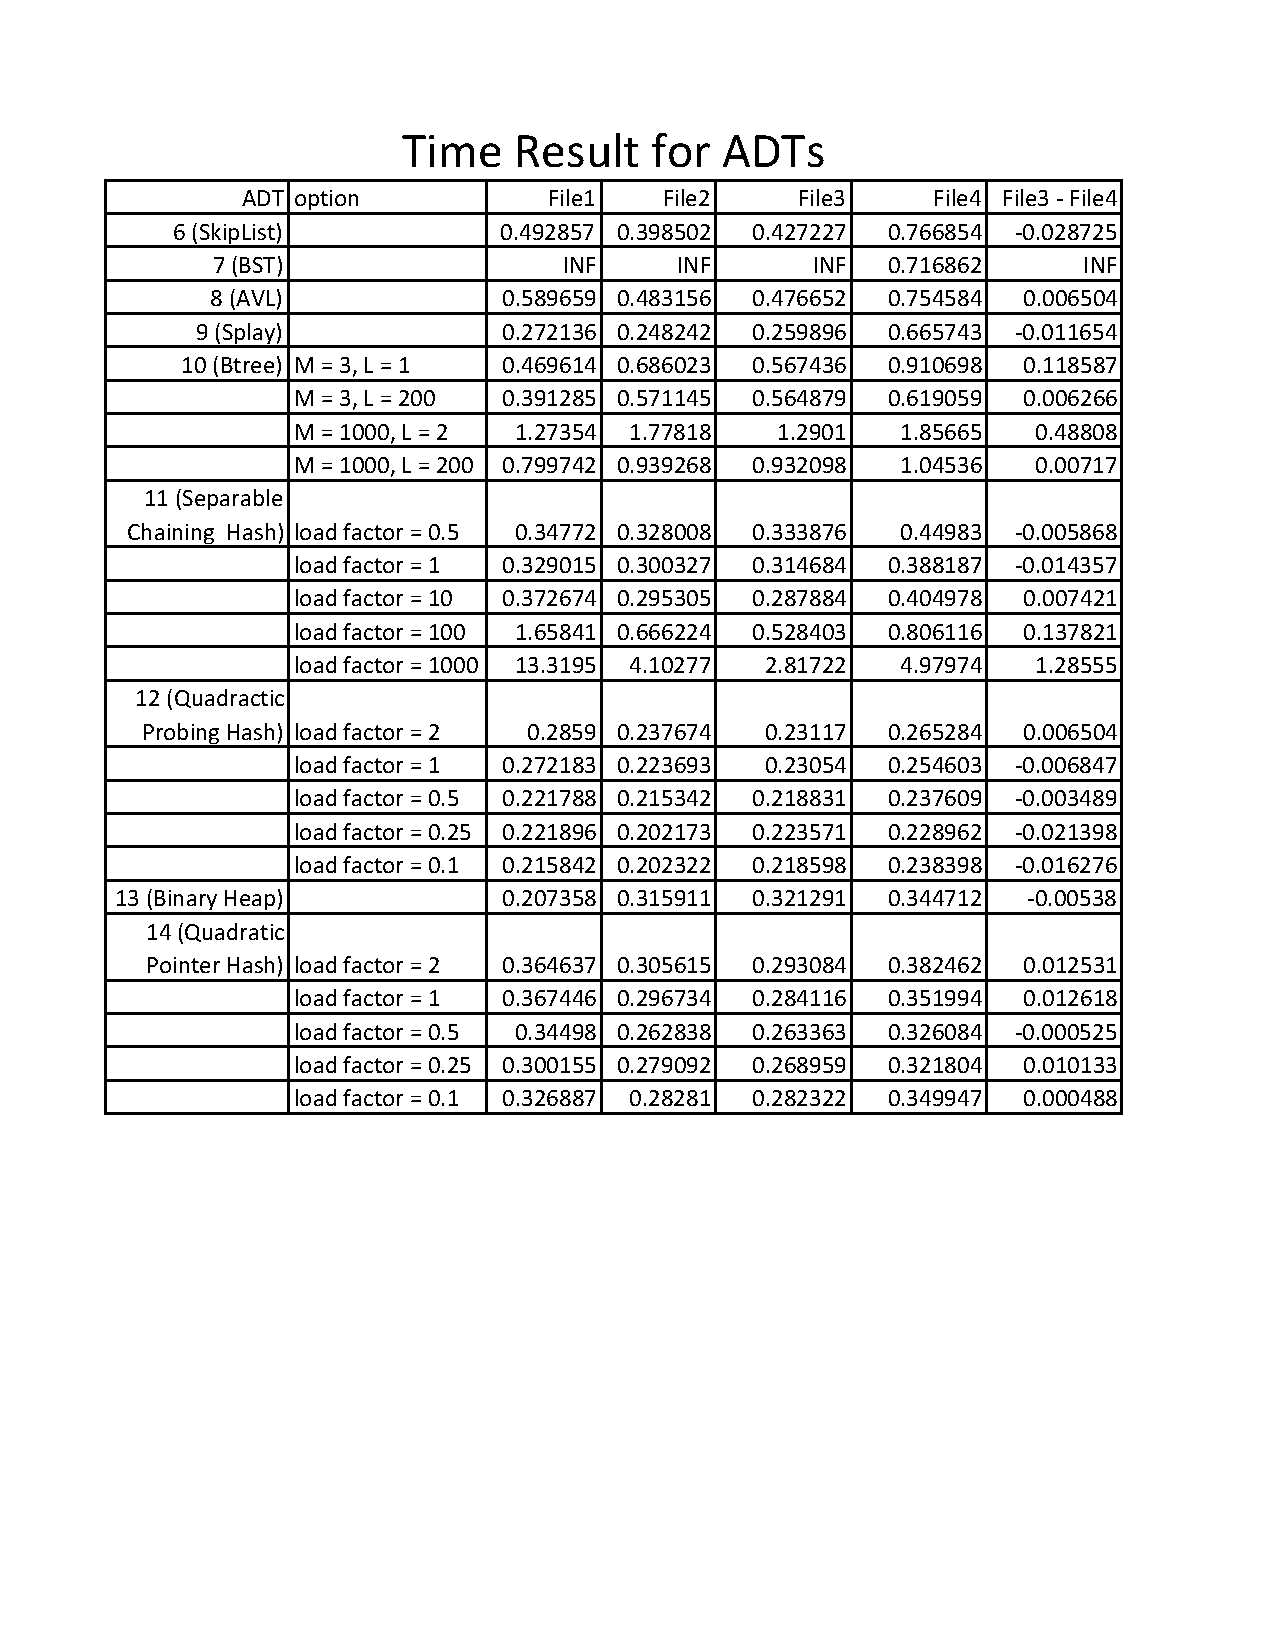
\includegraphics{timetest2_time}

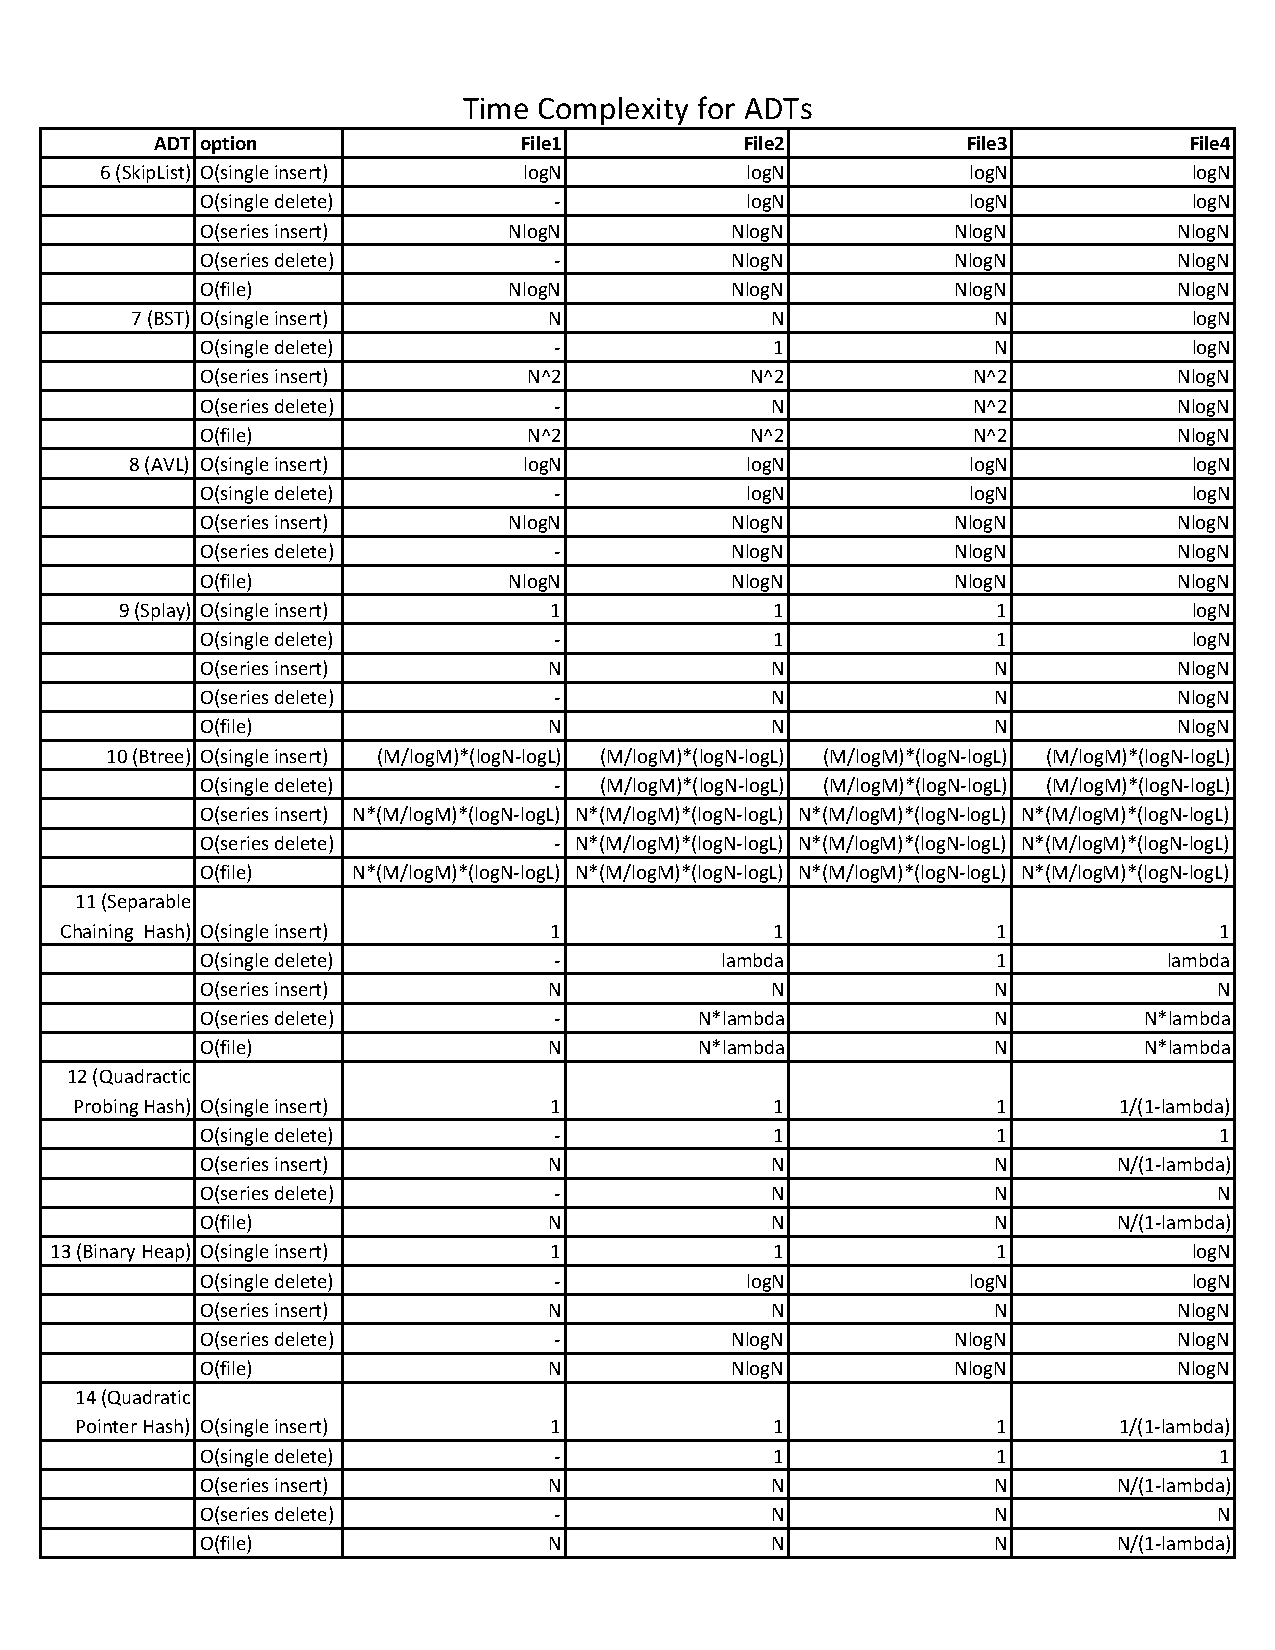
\includegraphics{timetest2_time_complexity}

\section{Part I: Analysis of each ADT on the Four
Files}\label{part-i-analysis-of-each-adt-on-the-four-files}

\subsection{BST}\label{bst}

The central idea of BST is to insert the new element at the leaf without
balancing. So when it is inserting numbers in order, it will usually
take O(N) to find the leaf, since it will form a big zig-zig format, in
other words, each node will only have the left sibling, and there is no
right sibling. But for file 4, for random insertion, we can assume the
BST will have a balanced structure, so the insert time will cost O(logN)
time.

In terms of deletion, time is largely different for file2 and file3.
Since our BST is head insertion, so when doing deletion, head deletion
will find the first value as the desired one. Then time complexity for
file2 is O(1), and it takes N time to find the last one, which is the
one to be deleted in tail deletion, so file3 has time complexity O(N)
for single deletion.

\subsection{AVL}\label{avl}

As a balanced binary tree, it will always take O(logN) to do either
insertion or deletion, and sometimes it needs one or two times rotation
when zig-zig or zig-zag come into being. But compared to O(logN) it is
much smaller, so the total time complexity for file1-4 are all O(logN)
for insertion and deletion.

But when we are actually comparing the time differences between these
four files, we find that the time of file2 and 3 are almost identical,
while file 1 is a bit larger, file 4 is the largest. I think for file 1,
it is due to the result of \(\sum^{2N}_{i=1}log(i)\) is larger than
\(2*\sum^{N}_{i=1}log(i)\).

\subsection{Splay}\label{splay}

The time complexity for splay insertion are all O(1) for file1-3, since
for head insertion, when we are inserting an element each time, we first
insert into the right child of the root node, and then do one rotation
to get the result. So it only takes 2 operations, which is clearly O(1).
But for random insertion, file4, it usually takes O(logN) to find the
right place to insert. Although the design of splay tree will not
balance the tree deliberately, the random insert order will balance it,
since every number will go up to the root, making the structure
balanced, so file4 needs much more time.

In terms of deletion, I first explain file2, which is head deletion. It
only involves one operation, just delete it. We do not need to rotate
the tree to place the element to be deleted to the root, since it is
already in the root. when we are doing tail deletion, which is file3, at
the first deletion, we first rotate the tree such that the largest
element, 250000, will be in the root. What's more, we will get a tree
top-down from 250000 to 1. It means that after the first deletion, in
subsequent deletions, we only need to delete the root order, which will
have the same operations for that of file2. So compared with file2, it
only has one more step: rotate the splay tree from 1 to 250000 to from
250000 to 1. The time of rotating is much less than deleting, so time
complexity for file3 of individual deletion is also O(1). Of course, for
file4, the deletion is O(logN), which is the time needed to find the
element.

\subsection{BTree}\label{btree}

The time complexity for BTree in terms of is
\(O(\frac{M}{logM}(logN-logL))\). The reason is: The height of the BTree
is \(log_M(N/L)\), which is \(\frac{1}{log(M)}(log(N)-log(L)\). Also, at
each level, we need to determine which children we should select: the
comparison takes (M-1) times. So finally the total average time will be
\(\frac{M-1}{logM}(logN-logL)\).

The time of deletion is the same as that of insertion, for the same
reason.

Now I can discuss the impact of M and L on the time complexity. Since
\(\frac{M}{logM}\) is monotonically increasing, so for \(M = 3\) vs
\(M = 1000\), the latter will take much more time to locate a particular
value. For the value of L, the time is monotonically decreasing with the
increase of L, and we can see the result matches my explanation.

Here I will continue to explain the difference between file2 and file3.
At first sight there is almost no difference between them: I think it
should be identical between head deletion and tail deletion. But when I
dip into the code, I find something interesting:

\begin{Shaded}
\begin{Highlighting}[]
\NormalTok{BTreeNode* InternalNode::remove(}\DataTypeTok{int} \NormalTok{value)}
\NormalTok{\{  }\CommentTok{// to be written by students}
  \DataTypeTok{int} \NormalTok{pos; }\CommentTok{// will be where value belongs}
  \KeywordTok{for}\NormalTok{(pos = count - }\DecValTok{1}\NormalTok{; pos > }\DecValTok{0} \NormalTok{&& keys[pos] > value; pos--);}
  \CommentTok{//.....}
\NormalTok{\}}
\end{Highlighting}
\end{Shaded}

When we are searching for values in terms of remove, we first look at
the last one, and then the one before the last one, so on so forth. This
means that, tail deletion will be in favor of this, finding the target
at first search, while head deletion can find the result only at the
end. This can explain the difference between file2 and file3, which is
totally due to deletion order. I also noticed that with the increase of
L and decrease of M, the difference is smaller: it is because a smaller
M can lead to finding the last element in each internalNode easily, and
a larger L will result in less height, so we can get the target with
less search. All of these will give us a smaller time difference between
file2 and file3.

\subsection{Separable chaining hash}\label{separable-chaining-hash}

For separable chaining hash, the performance is closely related to the
load factor. I claim it is because the time of deletion. But first let
me explain why insertion time complexity is O(1). Independent of load
factor, we are actually inserting the element at the head of each
linkedlist, so insertion only takes two operations, one is to find the hash
location, the second is to insert the element into the corresponding
linkedlist.

In terms of deletion, since the size is the total size divide the load
factor, so for each node, the linkedlist will contain elements identical
to the value of load factor. For head deletion, the linkedlist has to
traverse all the elements in the linkedlist, which is load factor
(\(\lambda\)). But for tail deletion, we can just find it at the
beginning of the linkedlist, so time complexity is O(2). From the time
complexity point of view, although they are all O(1), but the constant
before the time is significantly different from each other, and the
difference becomes larger when the load factor is larger. That is the
reason of difference of file2 and file3, and why the difference is
larger when load factor is over 10. Of course, load factor plays an important
role in the performance. I will discuss it in the final part.

\subsection{Quadratic probing hash}\label{quadratic-probing-hash}

Consider quadratic probing hash, for load factor 2 and 1, the program
need to rehash 2 and 1 times respectively to hold all the elements
inserted. For load factor 0.5, 0.25, 0.1, the ADT need not to rehash. So
it will need a little less time to do all the operations. And when we
are looking at the files, the result is as such: factor 2 and 1 needs
more time, and the time of other factors are almost identical. Things are
different for file 4. Since it is random insertion, it will have the chance
of collision, and the probability is \(1-\lambda\), then the
expectation will be \(\frac{1}{1-\lambda}\), which means it needs more time
to do all the operations.

I will talk more about the idea behind rehashing and size factor in the next part.

Sometimes we need to take into account the collision and clustering
problem. But here, our table size is very large, and quadratic hash
function also optimize to minimize the number of collisions.

\subsection{Binary heap}\label{binary-heap}

First I should note here, as a minimum binary heap can only find the
smallest value, so the deletion operation is only deleting the smallest
value, like what we have already seen in stack and queue, regardless of
the delete value. So the operation of file2 and file3 are essentially
the same.

Now since we are doing head insertion, so the time complexity is only
O(1), we just need to insert it at the end of the binary heap array, and
since it is already the biggest one, no swap is needed.

For deletion, we need to first remove the root item, which is the
minimum, and take the last value, which is the largest one, to the root.
Finally, we percolate the new root down, to the leaf level, since it is
the largest. It takes time O(logN). Since file2 and file3 are doing the
same operations (explained earlier), so there is no difference between
them.

\subsection{Quadratic probing pointer
hash}\label{quadratic-probing-pointer-hash}

It is just a pointer implementation of quadratic probing hash ADT. so
all the time complexity will be the same as quadratic probing hash. Of
course there is difference between their times, I will compare them in
the next part.

\section{Part II: Comparing ADTs with each
other}\label{part-ii-comparing-adts-with-each-other}

\subsection{Trees, Skiplist}\label{trees-skiplist}

There are many trees, and skiplist is also sharing the same inner logic
with trees. By giving the internalNodes, the search process becomes much
more simple. But the time complexity between them are still
significantly different. Let me compare them.

\paragraph{\texorpdfstring{\emph{AVL and
Skiplist}}{AVL and Skiplist}}\label{avl-and-skiplist}

Both of them are O(logN) in this problem, and are all implemented by
pointers. But there is a little difference between: in AVL, to keep the
binary tree balanced, we sometimes need to rotate the tree once or
twice, but for skiplist, we only need to find an appropriate location to
build the node. It means that AVL does one more step than skiplist
sometimes, so the time of it is a little longer.

\paragraph{\texorpdfstring{\emph{Splay
tree}}{Splay tree}}\label{splay-tree}

Although in general the average time complexity for splay is O(logN)
(reflected in file4), file2 and file3 only takes O(1) time complexity
due to its special order. But the time of file4 is close to AVL and
skiplist.

\paragraph{\texorpdfstring{\emph{BST}}{BST}}\label{bst-1}

In general, the average time complexity for BST should be O(logN) as
well (reflected in file4), file2 and file3 only takes O(N) time
complexity due to its special order, so I could not run the time out
because it is longer than 300 seconds, so I give it INF to indicate long
time. But the time of file4 is close to AVL and skiplist.

\paragraph{\texorpdfstring{\emph{BTree}}{BTree}}\label{btree-1}

Assume M = 3 and L = 1. By the equation \(O(\frac{M}{logM}(logN-logL))\)
given in the BTree part above, we know it is O(\(\frac{3}{log3}logN\)).
Since \(\frac{3}{log3} > 1\), then BTree performs worse than O(logN)
complexity. So the time of BTree is a larger than all the other trees.

\subsection{BTree for different M and
L}\label{btree-for-different-m-and-l}

I have already explained part of the BTree performance with respect to M
and L previously in the BTree part: The time complexity for BTree in
terms of is \(O(\frac{M}{logM}(logN-logL))\). The reason is: The height
of the BTree is \(log_M(N/L)\), which is
\(\frac{1}{log(M)}(log(N)-log(L)\). Also, at each level, we need to
determine which children we should select: the comparison takes (M-1)
times. So finally the total average time will be
\(\frac{M-1}{logM}(logN-logL)\). So with smaller M and larger L, it will
perform better.

The performance of BTree is a little complicated, since it is closely
related to the value of M and L, as well as the filled rate of BTree.
When BTree is almost full, although the height is small, we need to
compare our value in hand with all the M values in the internalNode to
decide which children to step into. For the worst case, we need to
compare M-1 times to find the children and key. Now the time is
\(O(\frac{M}{logM}(logN-logL))\), and sometimes it will be larger than
O(logN) if M is very large. For the extreme case, if M is equal to N, we
need to traverse the whole BTree, so the time complexity is \(O(N)\).

This reminds us of when BTree is useful. As I said earlier, when BTree
is almost full, the performance is not good. But when it is scarce, we
do not need to compare M-1 times at the internalNode level, so it will
be much faster.

\subsection{Hash table comparison}\label{hash-table-comparison}

There are three implementations of hash table here: Separable chaining
hash, Quadratic probing hash and Quadratic probing pointer hash. The
first one is implemented by linkedlist, and the last two are implemented
by vector, with one holding objects and the other holding pointers. I
will first explain the difference between the first one versus the other
two, and then the difference between the last two.

\paragraph{\texorpdfstring{\emph{Chaining vs
probing}}{Chaining vs probing}}\label{chaining-vs-probing}

It should be noted that each of them has upside and downside. For
separable chaining, we do not need to do rehash and have no chance of
collision, since linkedlist can absorb all these problems. For Quadratic
probing (pointer), we only have the advantage of locality of reference.
The concept of locality of reference means that, when we are asking an
object, the memory not only gives us the object, but also gives us the
memory block containing this object. In terms of vector and array in
C++, objects are stored contiguously in the containers, so there are
almost no cache misses, which will improve the performance.

So our question leaves us to compare which advantage outperforms the
disadvantage. At first sight the upside of chaining should dominate, but
it turns out that quadratic probing (pointer) is much faster. This
indicates that locality of reference saves much more time than time
waste on rehashing and collisions.

Another big difference is, for linkedlist, everytime we create a new
node, we need to use new to create a new pointer. But for array, we do
not need to do so: it has been initialized. Here chaining needs to use
new to create new node every time, but for probing, the only thing is
just fill the node with value, and rehash at an appropriate time. So
quadratic probing needs less time in this aspect as well.

\paragraph{\texorpdfstring{\emph{Quadratic probing vs Quadratic probing
pointer}}{Quadratic probing vs Quadratic probing pointer}}\label{quadratic-probing-vs-quadratic-probing-pointer}

The only difference between these two implementations are the first one
is a vector holding objects, while the second one is a vector holding
pointers. It can be seen from the constructor in each class. For objects
vs pointers, the differences can be discussing from these aspects: the
efficiency of copy constructor, the optimality of locality of reference.

For the copy constructor, if the copy constructor with respect to an
object is simple, which means it is not so complicated that copy needs
too much space and time, and is not polymorphic either, then this part
will not influence the efficiency too much. On the other hand, for the
locality of reference, if the program needs to iterate the object very
much often, then the performance will get significantly improved if it
can take advantage of the locality of reference.

For the comparison here, the object HashEntry is not complicated at all:
only consists of a HashObj and an EntryType. What's more, vectors of
pointers cannot take advantage of locality of reference: the program has
no idea of what the address of the the next pointer is, while vectors of
objects can easily predict the address of the next object, since vector
holds the objects contiguously. So in theory, the performance of
Quadratic probing hash should outperform Quadratic probing pointer hash.
The time validates my argument.

\subsection{Affects of different load
factors}\label{affects-of-different-load-factors}

I should note that, the load factor here is just a synonym of initial
size: we use load factor to choose initial size. The idea behind
rehashing and size factor is the trade off between time and space
complexity: we need to find a balanced size to minimize the time of
searching and inserting, as well as deleting. It does not mean that a
hash table with a very big size is good: we need to find the appropriate
size, since a big size hash table will need more time to locate a
particular element, and there will be too much space waste. When the
load factor is too small, we must rehash very frequently, and we are
more likely to get collisions, which will need more time to run.

So how to choose an appropriate value of load factor is very important.
We can decide the value by predicting our subsequent number of deletions
and insertions, to make it small enough, but can hold most the
operations we will do.

\subsection{Compare the performance of the Quadratic Probing hash with
QuadraticProbingPtr}\label{compare-the-performance-of-the-quadratic-probing-hash-with-quadraticprobingptr}

Please see Hash table comparison::Quadratic probing vs Quadratic probing
pointer. This section is above.

\end{document}
